\documentclass[conference]{IEEEtran}
\usepackage{cite}
\usepackage{amsmath,amssymb,amsfonts}
\usepackage{algorithmic}
\usepackage{graphicx}
\usepackage{siunitx}
\usepackage{textcomp}
\usepackage{xcolor}
\usepackage{multirow}
\usepackage{url}
\usepackage{listings}
\usepackage{epstopdf}
\usepackage{subcaption}
\usepackage[inkscapeformat=png]{svg}
\usepackage[font=small,labelfont=bf]{caption}

\graphicspath{ {./resources/} }
\epstopdfDeclareGraphicsRule{.gif}{png}{.png}{convert gif:#1 png:\OutputFile}
\AppendGraphicsExtensions{.gif}

\begin{document}

\title{Dynamic load balancing in distributed systems}

\author{\IEEEauthorblockN{Mihai Bojescu}
\IEEEauthorblockA{\textit{Masters in Artificial Intelligence and Optimisation} \\
\textit{Faculty of Computer Science of University ``Alexandru Ioan Cuza'' of Iași}\\
Iași, Romania \\
bojescu.mihai@gmail.com}
}
\maketitle

\begin{abstract}
    This document details what is load balancing, what is the dynamic load balancing strategy in distributed systems,
    possible architectures and challenges, case studies on Kubernetes and AWS ELB, and an experimental design created as a demonstration for the previously mentioned work.
\end{abstract}

\begin{IEEEkeywords}
    Load balancing, distributed systems, architectures, demonstration
\end{IEEEkeywords}

\section{Introduction}
    In distributed systems, load balancing is the act of distributing the workload across multiple nodes. Load balancing
is performed in order to make greater use of the available resources (such as I/O devices, memory, CPU, data), increase efficiency
of resources, lower response times, or to lower the costs of idle resources. Compared to simple load sharing, load balancing
aims to roughly evenly distribute the workload on the available nodes, which is a desired global optima of the system.

    Effective load balancing comes with many challenges, such as load estimation, load level comparison, system stability,
efficient task transfer, efficient messaging between nodes, peer selection, and more.

    Load balancing can be of two distinct types, based on the knowledge used to perform the balancing:

    \begin{enumerate}
        \item Static load balancing
        \item Dynamic load balancing
    \end{enumerate}

    Generally, load balancing is performed at 2 OSI layer levels: OSI layer level 4 and OSI layer level 7.

    In the sections below, both static and dynamic load balancing strategy will be detailed.

\section{Static load balancing}
    In static load balancing, prior knowledge about the compute nodes is required. Static load balancing is generally used
in systems where the task size is known and is predictable. In such scenario, the topology of the system is well-known ahead
of time, and ahead of the task execution. Tasks assigned to one node cannot be transferred to another one.
In general, static load balancing is rigid, but less complex to implement.

\subsection{Architectures and topologies}
    Static load balancing mainly follows 2 architectures:

    \begin{enumerate}
        \item ``Explicit'' balancing, using a load balancer in front of nodes \cite{b1}
        \item ``Implicit'' balancing, using a DNS and exposed nodes \cite{b3}
    \end{enumerate}

    The ``explicit'' balancing architecture aims to distribute traffic to nodes in a more controlled manner, giving
control to the application to perform this action.

    This presents multiple advantages:

    \begin{enumerate}
        \item Extracting the responsibility of traffic filtering away from the targeted application nodes
        \item Implementation is more accessible
        \item Multiple plug-and-play solutions already exist, such as NGINX, Apache, HAproxy
    \end{enumerate}

    And some disadvantages:

    \begin{enumerate}
        \item When the load balancer fails, the users don't have access to the application
        \item When the load balancer gets overloaded, the users will experience high latency
        \item The load balancer is an additional resource that needs to be managed
        \item The overhead is higher, as the load balancer might not be next to the application server
    \end{enumerate}
    
    \begin{center}
        \vspace{1em}
        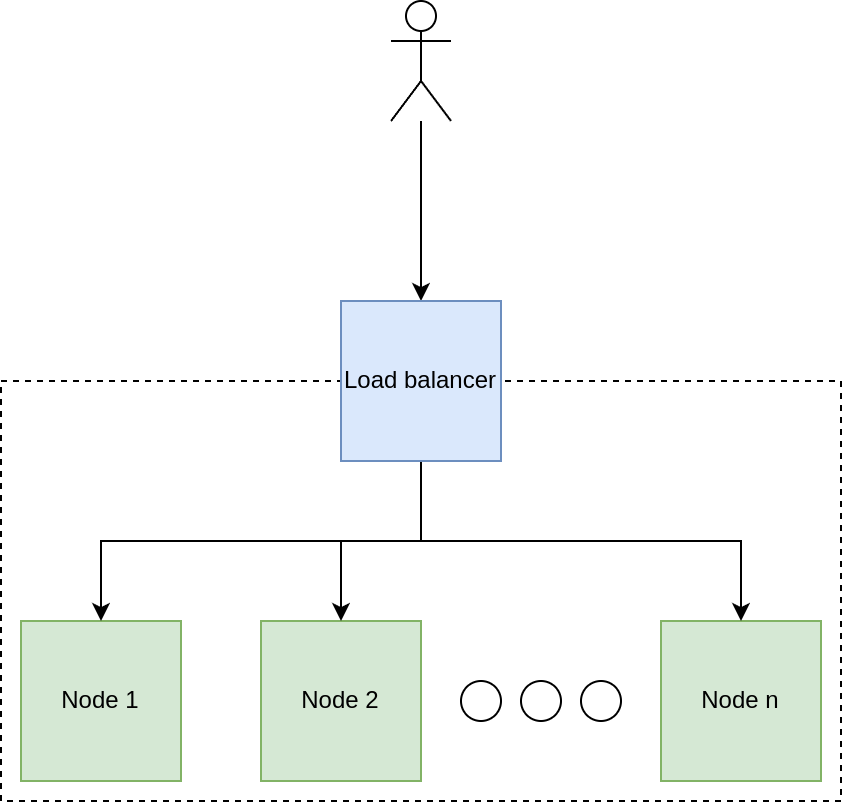
\includegraphics[width=0.4\textwidth]{traditional-load-balancing.png}
        \captionof{figure}{Explicit load balancing using a load balancer} \label{traditional-load-balancing}
        \vspace{1em}
    \end{center}

    The load balancer can also be swapped for a message broker, achieving the same effect. The architecture is more complex,
now relying on both a gateway and the message broker, but this allows for better availability.

    \begin{center}
        \vspace{1em}
        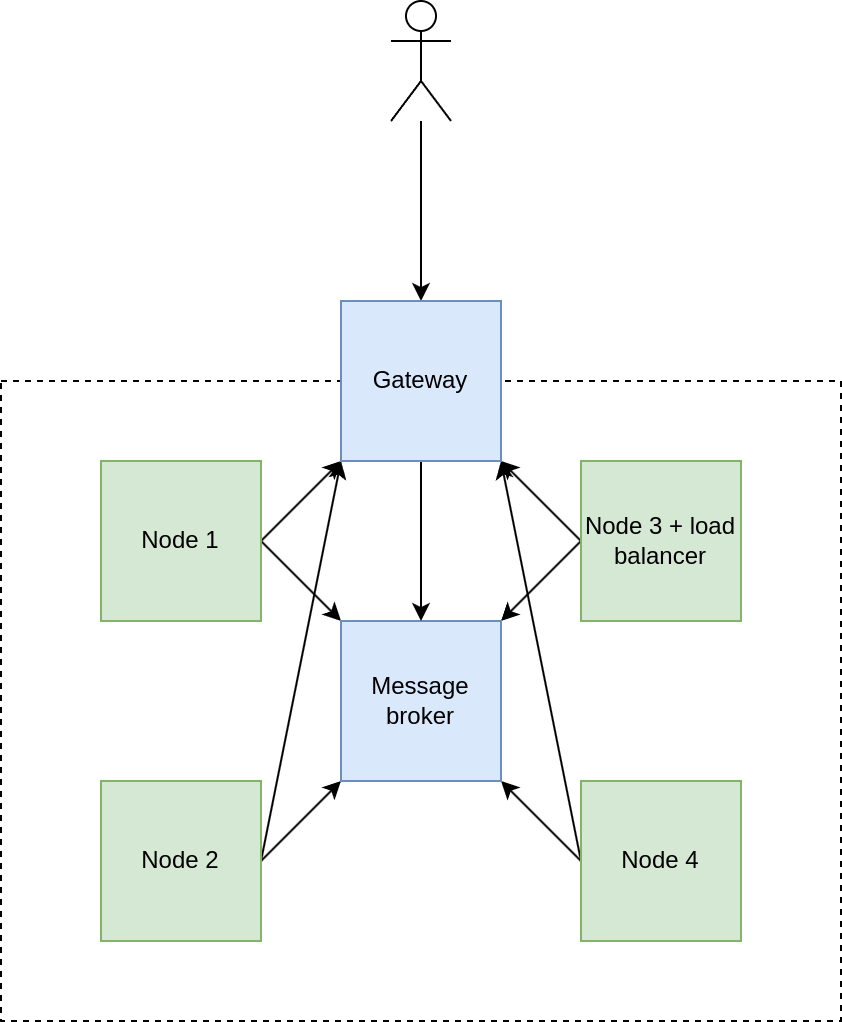
\includegraphics[width=0.4\textwidth]{message-broker-balancing.png}
        \captionof{figure}{Explicit load balancing using a message broker} \label{message-broker-load-balancing}
        \vspace{1em}
    \end{center}    

    The ``implicit'' balancing architecture aims to pass the load balancing task from a load balancer to a DNS server,
which will rotate addresses, in hopes of achieving even task distribution. This performs implicit load balancing, as the
client can decide wether to use the provided host, or to use another one from the DNS server response, assuming the DNS
server offers more than one response.

    This presents multiple advantages:

    \begin{enumerate}
        \item The design is even simpler than figure \ref{traditional-load-balancing}, as no load balancer needs to be managed and
        maintained
        \item It can be simpler to implement than figure \ref{traditional-load-balancing} and figure \ref{message-broker-load-balancing}
        \item The DNS control \textit{can be} outside of the application context (public DNS, for instance), which can reduce
        costs
    \end{enumerate}

    Along with the disadvantages from figure \ref{traditional-load-balancing}, the architecture also has the following disadvantages:

    \begin{enumerate}
        \item In instances where the DNS is not owned by the application developer, the owner of the DNS server can perform
        modifications without the developer's knowledge, leading to issues
        \item The users might not know what DNS server to use to access the application
    \end{enumerate}

    \begin{center}
        \vspace{1em}
        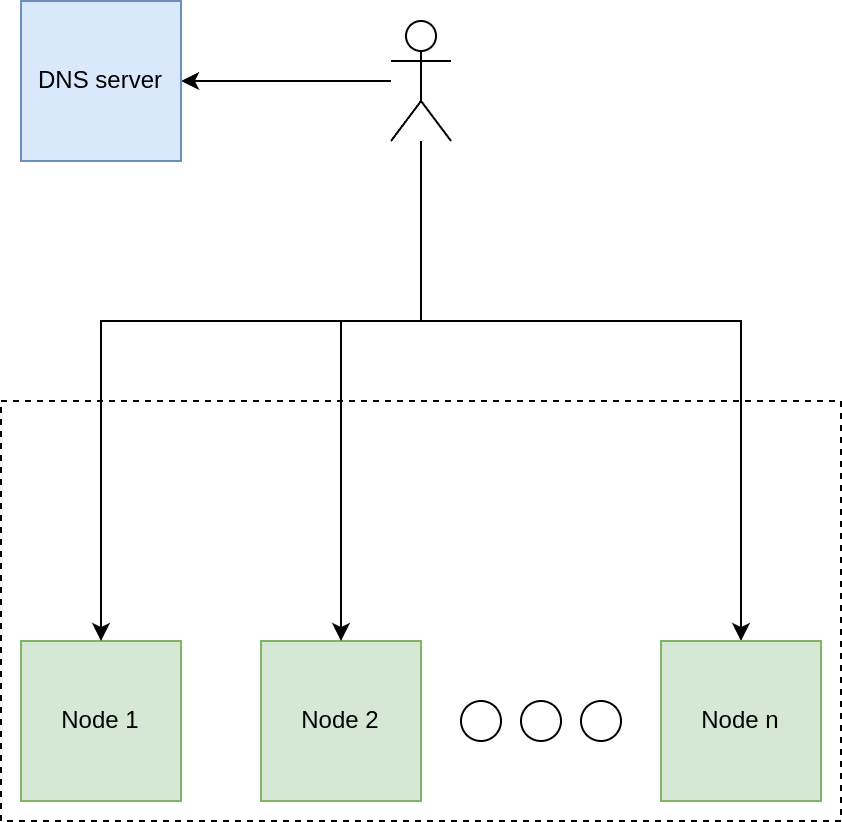
\includegraphics[width=0.4\textwidth]{dns-load-balancing.png}
        \captionof{figure}{Implicit load balancing using DNS} \label{dns-load-balancing}
        \vspace{1em}
    \end{center}

\subsection{Algorithms}
    In static load balancing, the following strategies are used:

    \begin{enumerate}
        \item Round-Robin method aims to evenly distribute tasks to each server,
        without taking in consideration the load of the server
        \item Random choice method aims to distribute tasks to different nodes, at random
        \item Hashing method aims to hash the url, and pass the request to a node that matches the hash
        \item Least connection method aims to send the request to the least full node that the node knows about,
        without taking in consideration the load of the server
        \item Weight distributed method aims to send the requests to based to a prior-set weighted node selection. 
    \end{enumerate}

    \begin{center}
        \vspace{1em}
        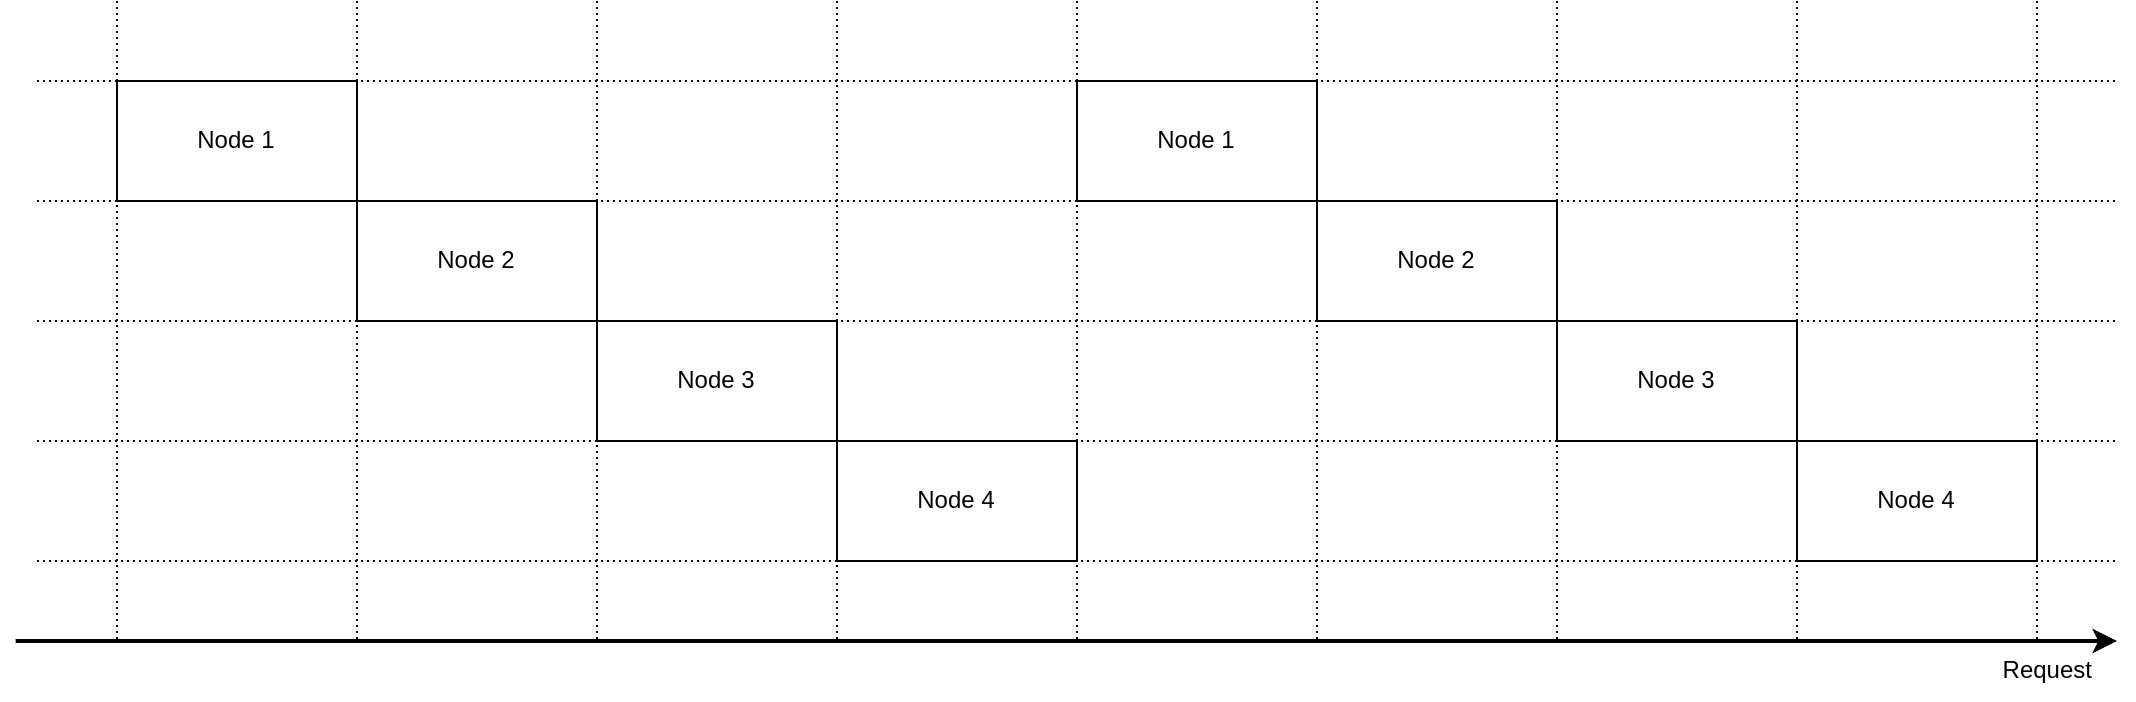
\includegraphics[width=0.5\textwidth]{round-robin-method.png}
        \captionof{figure}{Round-Robin strategy} \label{round-robin-strategy}
        \vspace{1em}
    \end{center}

    \begin{center}
        \vspace{1em}
        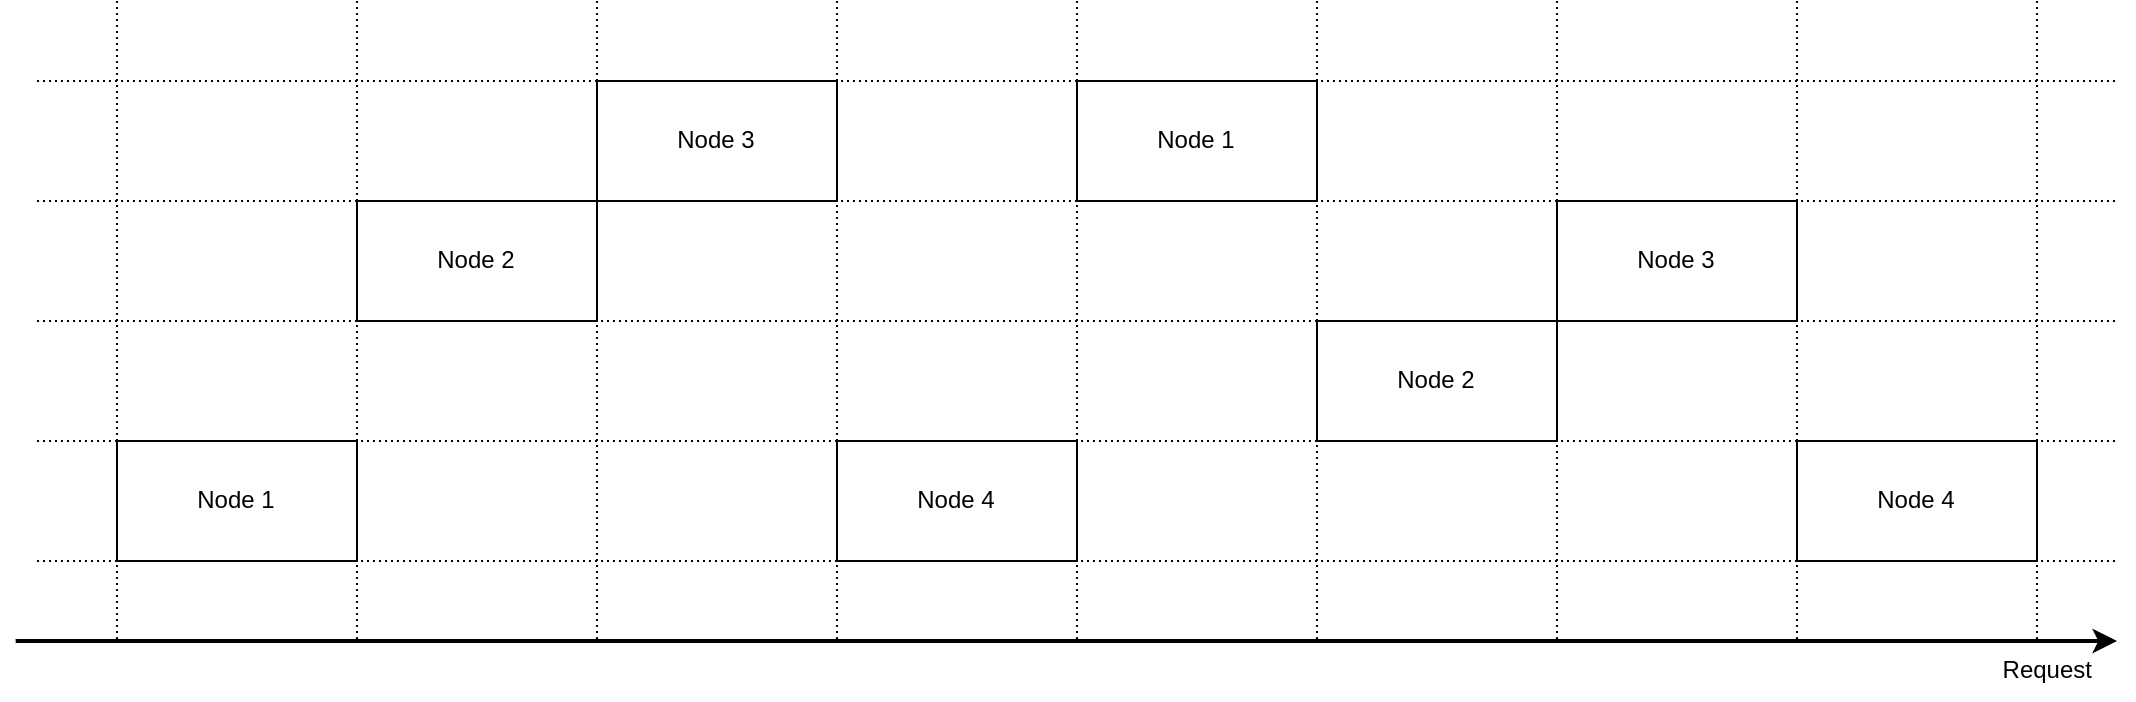
\includegraphics[width=0.5\textwidth]{random-method.png}
        \captionof{figure}{Random strategy} \label{random-strategy}
        \vspace{1em}
    \end{center}

\section{Dynamic load balancing}
    In dynamic load balancing, no knowledge of the system and tasks is required or assumed a priori. Tasks are dynamically
assigned, reassigned and distributed to the available nodes in the system without the prior input from the application developer.
The strategy is highly flexible and provides high availability, with generally more performance compared to the static load
balancing strategy. While the strategy has many advantages, it requires more resources, is prone to high chattiness, and
is more complex overall. 

    Various studies on dynamic load balancing, such as \cite{b2}, show that such strategy can increase the resource utilisation,
lower response times, increase availability and reduce costs. 

    Dynamic load balancing algorithms are varied, and an effective one must trade between the disadvantages listed above in
order to achieve good performance of the system. They range from simple comparisons to advanced statistical analysis to achieve
the desired system. Some well-known algorithms will be listed in the sections below, along with their use-cases.

\subsection{Architectures and topologies}
    Dynamic load balancing architectures don't overlap with static load balancing architectures in full, as the ``implicitly''
balanced architectures are not supported.
    
    \begin{enumerate}
        \item For the static ``explicitly'' balanced architecture, the load balancer must take into account the load of each node before assigning tasks
        \item For the static ``implicitly'' balanced architecture, the DNS server must account for individual node load. This effectively makes the
        architecture an ``explicitly'' balanced one.
    \end{enumerate}

    Along the two aforementioned architectures, the strategy allows for a decentralised one, supported by the task transfer
option of the dynamic load balancing strategy and by individual node load balancing. The architecture allows nodes to be independently scaled,
thus achieving higher resource utilisation efficiency.

    \begin{center}
        \vspace{1em}
        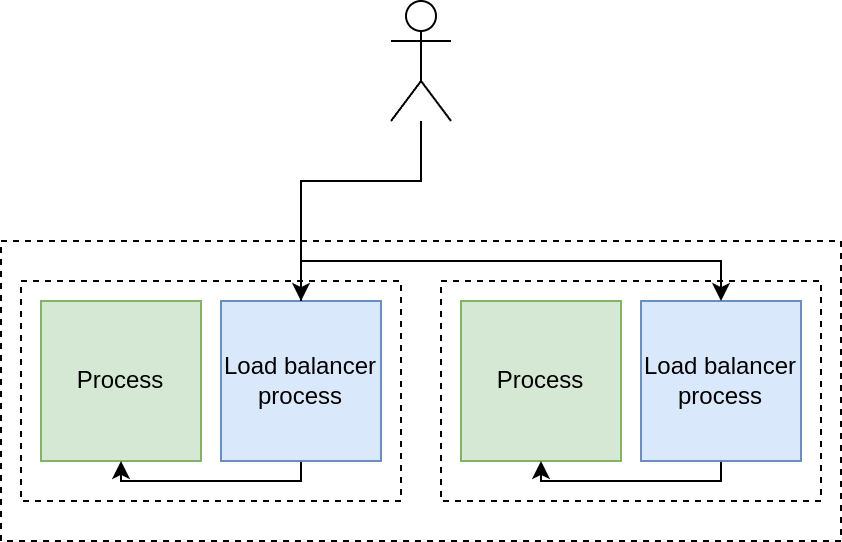
\includegraphics[width=0.4\textwidth]{internally-load-balanced-node.png}
        \captionof{figure}{Internal representation of decentralised, dynamic load balanced nodes} \label{internally-load-balanced-node}
        \vspace{1em}
    \end{center}

    \begin{center}
        \vspace{1em}
        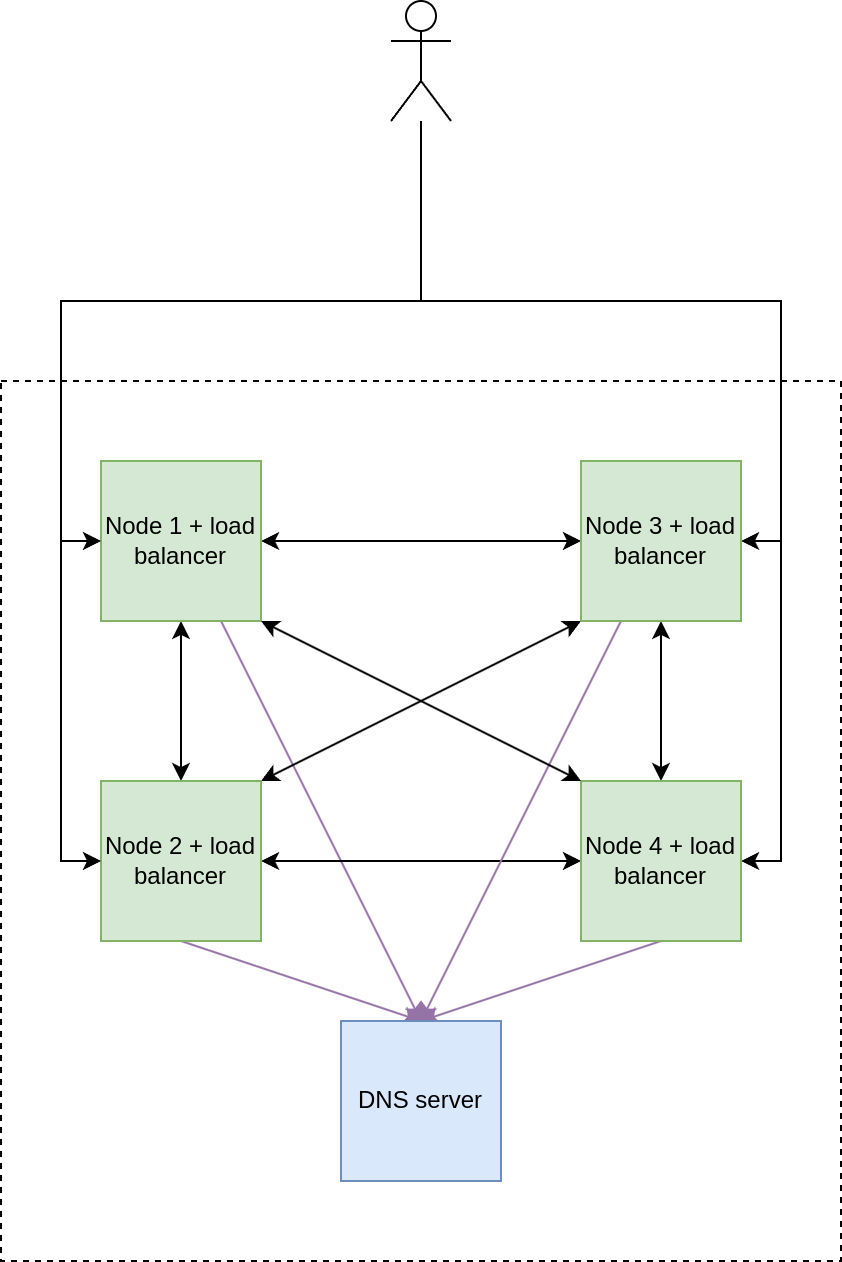
\includegraphics[width=0.4\textwidth]{decentralised-load-balanced-system.png}
        \captionof{figure}{Decentralised, dynamically load-balanced system, using internally, dynamic load balanced nodes} \label{decentralised-load-balanced-system}
        \vspace{1em}
    \end{center}

\subsection{Algorithms}
    Dynamic load balancing are rather diverse, can take multiple parameters such as CPU load average, used memory, tasks in
queue and response times.

    Many algorithms are based on one of the following ones:

    \begin{enumerate}
        \item Least compute-loaded method
        \item Least response time method
        \item Least bandwidth used method
        \item Least packets used method
    \end{enumerate}

    The algorithms try to achieve the same global optima in different ways, and should be used depending on the specific
use-cases, some of them being:

    \begin{enumerate}
        \item Least compute-loaded method should be used for tasks such as video transcoding, AI workloads, CI/CD operations
        \item Least response time method should be used for tasks such as video and audio calls, stock markets, online games
        \item Least bandwidth used method should be used for tasks such as video streaming, cloud storage, CDNs
        \item Least packets used method should be used for tasks such as chat applications, external load balancers for DDoS mitigation
    \end{enumerate}

    Each algorithm uses metrics from the available nodes to perform load balancing effectively. Depending on the system, the
metrics can be pushed to the balancer, or pulled by it. Systems that use the push method tend to be
most chatty and have the least latency, while the pulling ones have ones are the polar opposite.

\section{Case studies}

\subsection{Case studies: Kubernetes}
    Kubernetes is a well-known open-source platform for building highly-available, highly-scalable and platform-agnostic web applications.
Pods can communicate between each other using the overlay network, without the need for NAT and without regard of running
on different nodes. The overlay network provides a flat IP address space, which eases communication.

    Kubernetes supports both static and dynamic load balancing across the nodes, depending on the given configuration.
By default, static load balancing is used.

    Architecturally, Kubernetes works similarly to figure \ref{traditional-load-balancing}, where a load balancer performs
traffic management. The load balancer (ClusterIP, NodePort, LoadBalancer) is individually-scalable in order to provide
better uptime.

    Kubernetes load balancers can perform the balancing at both OSI layer 4 and OSI layer 7, depending on the configuration.

    An example of load-balanced system configuration for Kubernetes is the following:

    \begin{center}
        \lstset{
            aboveskip=3mm,
            belowskip=3mm,
            showstringspaces=false,
            columns=flexible,
            basicstyle={\small\ttfamily},
            numbers=none,
            numberstyle=\tiny\color{gray},
            keywordstyle=\color{blue},
            commentstyle=\color{dkgreen},
            stringstyle=\color{mauve},
            breaklines=true,
            breakatwhitespace=true,
            tabsize=3
        }
        \begin{lstlisting}
    apiVersion: extensions/v1beta1
    kind: Ingress
    metadata:
    name: calendar-ingress
    spec:
    tls:
    - hosts:
        - calendar.example.com
        secretName: calendar-secret
    rules:
    - host: calendar.example.com
        http:
        paths:
        - path: /api/events
            backend:
            serviceName: events-svc
            servicePort: 80
        - path: /api/calendars
            backend:
            serviceName: calendars-svc
            servicePort: 80
        \end{lstlisting}
        \captionof{lstlisting}{Code example for a Kubernetes load balanced system} \label{kubernetes-load-balancing-example}
    \end{center}

    The resiliency of the system highly depends on the configuration of the cluster.

\subsection{Case study: AWS ELB}
    AWS ELB is a load balancer often used when building projects using the Amazon Web Services Cloud platform. The system
follows an architecture similar to figure \ref{traditional-load-balancing}. Similarly to Kubernetes, the system is individually
scalable and the scaling is handled implicitly by AWS unlike Kubernetes which perform  scaling explicitly using configuration
files.

    The solution is paid and closed-source, thus it does not permit auditing. As per AWS, AWS ELB can perform load balancing
both at OSI layer level 4 and OSI layer 7. The solution is also very well integrated with existing AWS products, such as EC2,
EKS and ECS.

    Performance auditing can be performed using ``siege'' or Apache ``ab''. Since the system is scalable, it is very resilient
to large number of requests.

\section{Experimental study: Building a decentralised, dynamically load balanced system}
    In this section, an experimental study will be detailed on building a decentralised, dynamically load balanced system
from start to finish. The targeted use-cases for such systems are CI/CD systems and batch processing workers, which need
to balance their compute evenly in order to achieve optimal system efficiency. The system can be used on other types of
workloads while still offering good efficiency, but might not be the best choice.

    The system includes the following components:

    \begin{enumerate}
        \item An OSI layer 7 load balancer
        \item A frontend application used to view the metrics of the node, which are used by the load balancer
        to perform the task placement
    \end{enumerate}

    The load balancer process polls a DNS server for peer nodes each second, which will be later used for passing tasks
when the node is compute-overloaded.

    For the balancing algorithm, a ``least compute-loaded method'' was applied. When a HTTP request is received by the
balancer, it queries at most $n$ nodes (configurable) for their metrics, and picks which has the most compute power available.
 
    Architecturally, the system is the same as figure \ref{decentralised-load-balanced-system}, where each node in the system
follows figure \ref{internally-load-balanced-node} for its components. The system was initially thought to work for containerised
applications using Docker, but can be applied to systems that don't have such prerequisite available.

\subsection{Experiments}

    The testing methodology was the following:

    \begin{enumerate}
        \item Apache ``ab'' CLI - a well-known HTTP API stress testing tool - was used
        \item A total of 20000 requests were sent in a session
        \item A total of 1000 requests were sent concurrently
        \item Tests were repeated 5 times
    \end{enumerate}

    When tested against a homogenous compute environment with two virtual machines, with each machine:

    \begin{enumerate}
        \item Having 2vCPUs and 1GB of RAM
        \item Running an application and a load balancer in Docker
    \end{enumerate}

    The results were:

    \begin{center}
        \centering
        \begin{tabular}{l|r|r|r}
            Metric & Min & Mean & Max \\
            \hline
            Latency & 33ms & 1131ms & 2381ms \\
            \hline
            CPU load average & 0.98 & 1.54 & 2.01 \\
            \hline
            Used memory (load balancer) & 109MB & 120MB & 132MB \\
        \end{tabular}
        \captionof{table}{Homogenous, dynamically load balanced system metrics for experimental study} \label{homogenous-nodes-metrics}
    \end{center}

    \begin{center}
        \vspace{1em}
        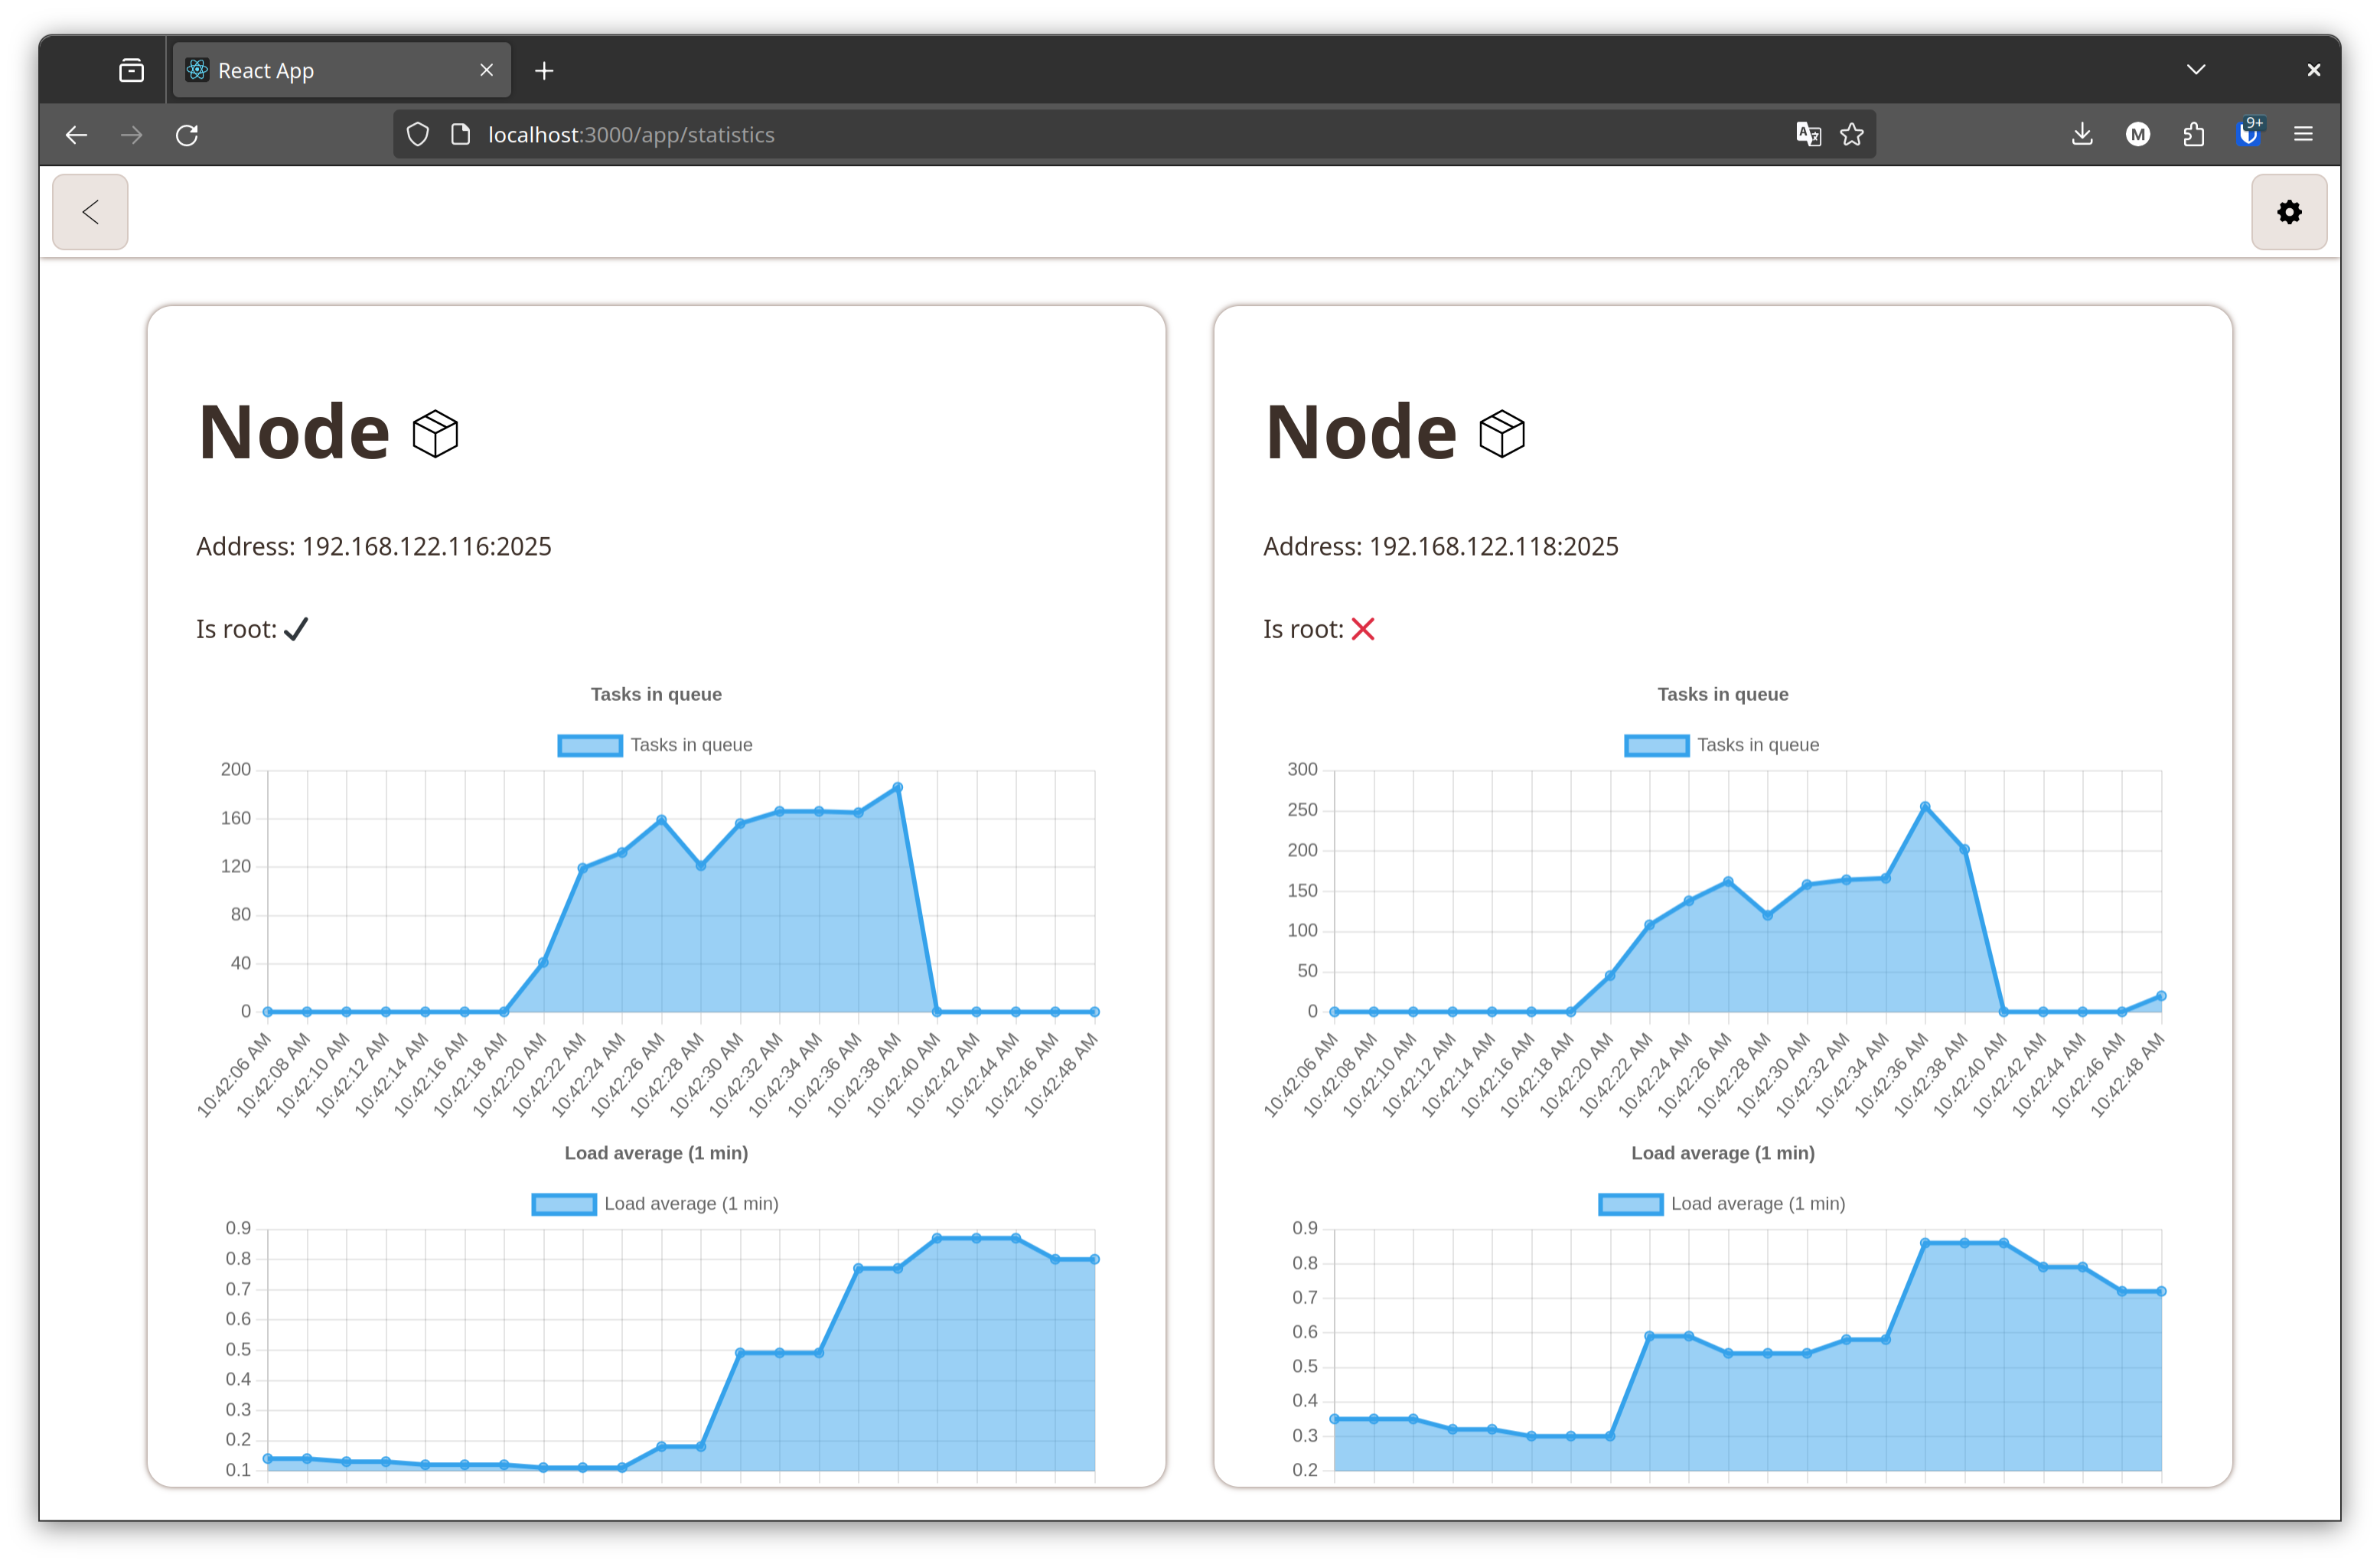
\includegraphics[width=0.4\textwidth]{homogenous-load-balancing-example.png}
        \captionof{figure}{Homogenous, dynamically load balanced system charts} \label{homogenous-load-balancing-example}
        \vspace{1em}
    \end{center}

    When using three heterogenous nodes - a laptop with an Intel Core i7 1260p processor, a BCM2711 SoC SBC, and a smartphone
with a Qualcomm Snapdragon 8 gen 3 processor, all running under a WireGuard VPN - the results were:

    \begin{center}
        \centering
        \begin{tabular}{l|r|r|r}
            Metric & Min & Mean & Max \\
            \hline
            Latency & 129ms & 582ms & 3527ms \\
            \hline
            CPU load average & 1.43 & 1.86 & 2.71 \\
            \hline
            Used memory (load balancer) & 176MB & 179MB & 182MB \\
        \end{tabular}
        \captionof{table}{Heterogenous, dynamically load balanced system metrics for the experimental study} \label{heterogenous-nodes-metrics}
    \end{center}

\subsection{Future work}
    The experimental study system presents some issue regarding connections being reset, issue which needs revised. Another
area which could use improvement is using push metrics instead of pull metrics for the load balancer, which can be used to
further improve efficiency and reduce system chattiness.

    Other areas of improvements include switching from Node.JS with Typescript to a statically compiled, high-performance
language such as C++ or Rust, improving logging, and adding support for more workload types.

\section{Conclusions}
    Dynamically load balanced systems aim to improve the performance and efficiency of distributed systems. Building effective
algorithms is not trivial and requires efficient communication between nodes for the system to work as intended.

    Architecturally, dynamic load balanced systems allow for more options than their static load balanced counterparts, which
is an added benefit.

    Since nodes can know the state of other nodes in the system, they can perform task transfers to make utilise the resources
more efficiently. Using this, a more decentralised system architecture can be achieved, which is more resilient to downtime.
This paper includes such a system built from scratch as an experimental study on this topic.

\begin{thebibliography}{00}
    \bibitem{b1} Ali M. Alakeel. ``Guide to Dynamic Load Balancing in Distributed Computer
    Systems''. IJCSNS International Journal of Computer Science and Network Security, VOL.10 No.6,
    June 2010
    \bibitem{b2} Z. Khan, R. Singh, J. Alam, and R. Kumar. ``Performance Analysis
    of Dynamic Load Balancing Techniques for Parallel and Distributed
    Systems''. International Journal of Computer and Network Security,
    vol. 2, no. 2, February 2010.
    \bibitem{b3} V. Cardellin, M. Colajanni, P. Yu. ``Dynamic Load Balancing On Web-Server Systems''. IEEE Internet Computing,
    June 1999.
    \bibitem{b4} Karen D. Devine a, Erik G. Boman, Robert T. Heaphy , Bruce A. Hendrickson,
    James D. Teresco,1 , Jamal Faik, Joseph E. Flaherty, Luis G. Gervasio. ``New challenges in dynamic load balancing''.
    Elsevier Applied Numerical Mathematics 52 (2005) 133-152, October 2004.
    \bibitem{b5} \url{https://www.nginx.com/blog/nginx-plus-ingress-controller-kubernetes-load-balancing/}
    \bibitem{b6} \url{https://docs.aws.amazon.com/elasticloadbalancing/latest/network/introduction.html}
    \bibitem{b7} \url{https://docs.aws.amazon.com/elasticloadbalancing/latest/application/introduction.html}
\end{thebibliography}

\end{document}
